\section{Background: Serverless Computing}\label{sec:background}

%data size as a criteria for the offloading decision
\begin{figure*}[bp]
	\centering
	\captionsetup[subfigure]{width=0.494\linewidth}
	\subfloat[Both \textit{feature extraction} and \textit{matching} compose a single service (fEM); mobile devices (md) are unable to offload fEM to SEP A, whose resources have been allocated to other functions; computation is offloaded to SEP B with one (1x) \textit{HTTP request} per video frame.\label{fig:Mobile_Computation_Offloading_F1}] {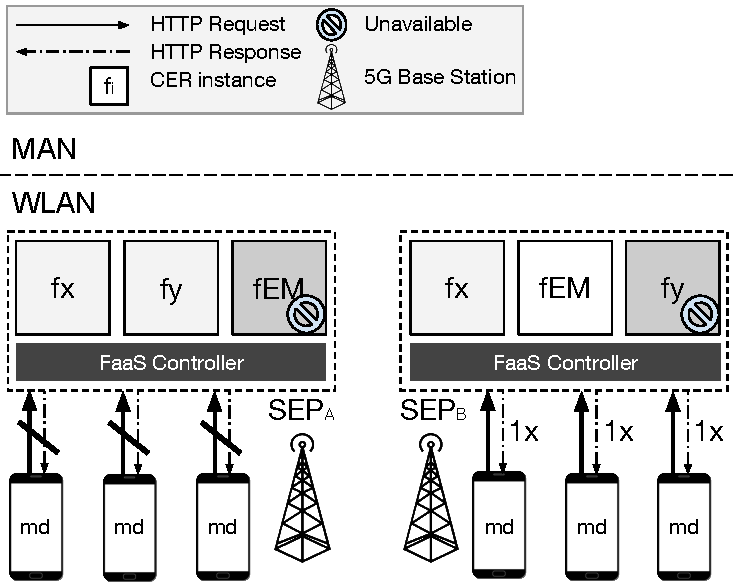
\includegraphics[width=0.494\textwidth]{Figs/Mobile_Computation_Offloading_F1.pdf}}
	~
	\captionsetup[subfigure]{width=0.504\linewidth}
	\subfloat[Data-intensive \textit{feature extraction} (fE) is provided by SEP$_A$ and SEP$_B$, while \textit{feature matching} (fM) is provided by SEP$_B$ and a Regional SEP (SEP$_R$). In total, computation is offloaded with two (2x) \textit{HTTP requests} per video frame, plus one (1x) inter-platform request (SEP$_A \rightarrow $SEP$_{B|R}$ and SEP$_B \rightarrow $SEP$_{R}$).\label{fig:Mobile_Computation_Offloading_F2}] {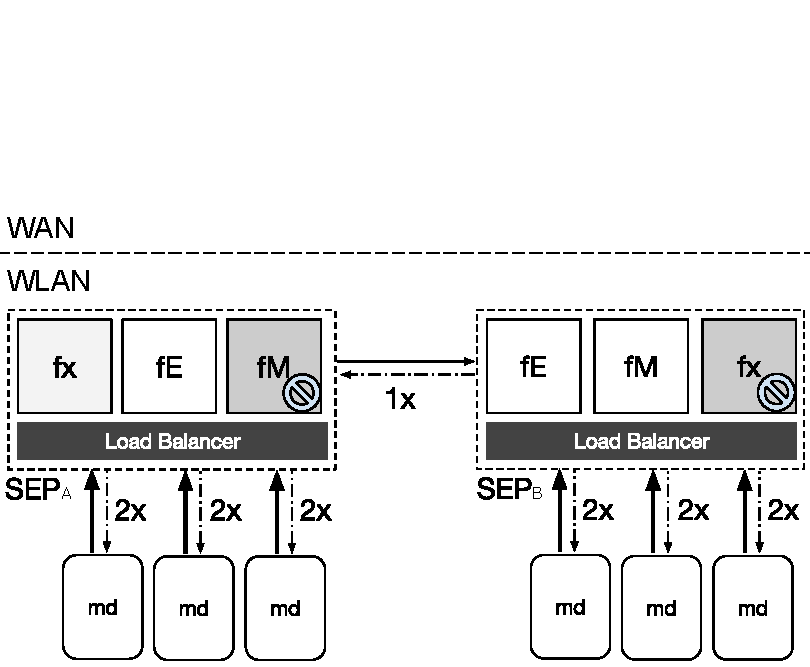
\includegraphics[width=0.504\textwidth]{Figs/Mobile_Computation_Offloading_F2.pdf}}
	\caption{\textit{Feature extraction} and \textit{matching} functions from the AR example forming a single function (a) and two fine-grained functions (b)} \label{fig:Mobile_Computation_Offloading}
\end{figure*}

%To address the characteristics of edge computing nodes, an edge platform must manage its resources very efficiently, which means provisioning and allocating resources only when they are needed. 

Serverless computing~\cite{Lloyd18serverless,Roberts:2018} is mainly associated with two concepts: of applications that rely on third-party cloud services for handling business logic and state (also known as \textit{Background-as-a-Service}); and that of applications for which server-side logic is still written by application developers, but, unlike traditional architectures, runs in stateless compute containers that are event-triggered
%, ephemeral (may only last for one invocation), 
and fully managed by a third party (also known as \textit{Functions-as-a-Service}, or FaaS).

In the FaaS model, application logic is implemented as functions, which may be written in various languages and exposed as web services. Functions are packed along with dependencies (e.g., modules, libraries, and other resources). Upon invocation, a \textit{containerized execution runtime} (CER) is reused from previous execution (warm container) or made available (new container) within milliseconds, thanks to the container technology. In particular, keeping containers \textit{warm} for a period of time prevents the CER initialization overhead (also known as \textit{cold start}) for subsequent requests. 


%containerized runtime instances (e.g., NodeJS, Python) are made available on demand within milliseconds, thanks to the container technology. 

%Functions can be executed just once, frequently, or concurrently. After completion, containerized runtime instances may remain idle (warm) for a short period of time before been reused or released.

%Upon invocation, a \textit{containerized execution runtime} (CER) is reused from previous execution (warm container) or made available (new container). In particular, keeping containers \textit{warm} for a period of time prevents the CER initialization overhead (also known as \textit{cold start}) for subsequent requests. 

\begin{figure}[tbp]
	\centering
	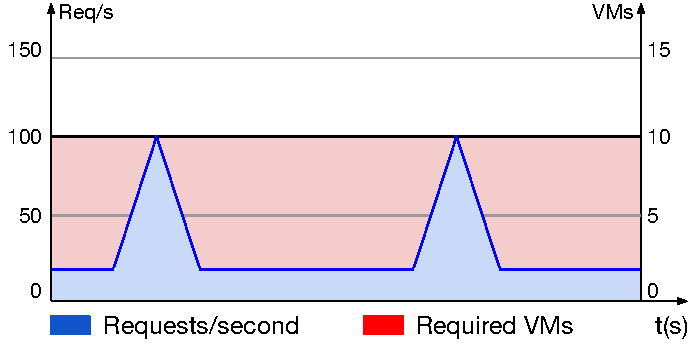
\includegraphics[width=0.9\linewidth]{Figs/IaaS_vs_FaaS}
	\caption{Inconsistent traffic pattern / Conventional IaaS deployment (adapted from~\cite{Roberts:2018})}
	\label{fig:IaaS_vs_FaaS}
\end{figure}

In comparison with a conventional \textit{Infrastructure-as-a-Service} deployment (Figure~\ref{fig:IaaS_vs_FaaS}), %a serverless architecture implies the automated provisioning and management of resources needed by the application. In particular, 
the FaaS model ensures resources (i.e., containers) to be allocated when actually needed. Whilst the use of virtual machines (VMs) enables applications to share physical resources, the FaaS model exploits the container technology to deliver the following advantages~\cite{GarrigaMendonca2017}:

\begin{itemize}
    \item a single operating system is shared among concurring CER instances from one or more functions; and
    \item functions are promptly deployed and scaled in reaction to demand without preallocating computational resources.
\end{itemize}

FaaS-based platforms (e.g., AWS Lambda~\cite{AWSLambda}) also enforce limitations to the function package size and execution time by design. Due to its characteristics, this execution model enables an efficient usage of computational resources, which is particularly important to cope with the resource limitations of edge platforms and to allow edge-based solutions to scale. 


%The achieve efficiency is particularly important in the context of fine-grained edge nodes exhibiting limited computational and storage resources. 

%a higher number of concurring functions~\cite{}.

%

%Also, users are billed by the actual usage of resources (pay-as-you-go). This model may give edge infrastructure providers a .

%\subsection{Edge Infrastructure and Architecture}

%Regardless of...

